\chapter{Conclusions}\label{cap.conclusions}



In this thesis we studied deep learning techniques and their application in a tracking algorithm. We included an object detector and a person re-identification module based on those techniques and we implemented a tracking algorithm.

This tracking algorithm, takes the detections of the object detector and computes the optical flow on the sequences. When it misses some pedestrians it can preserve their identity with a person re-identification module.

Finally we evaluated our algorithm in a well-known challenge, MOT16, and analyses its performance and timing capabilties on it. The algorithms performs reasonably well in sequences of high frame rate and resolution, but in the opposite sequences, low frame rate and resolution the performance drop dramatically. This is happens beacause our algorithm rely on points with high texture, with a low resolution there are less points with this characteristics. Also, we have problems with people who wear low texture or are away from the camera, as we can oberve in figure \ref{Fails1}. The low frame rate, penalize the matching capabilites between frames, it produces wrong matches between images, therefore, wrong displacements.




\begin{figure}[H]
		
\centering

\subfigure[High texture person.]{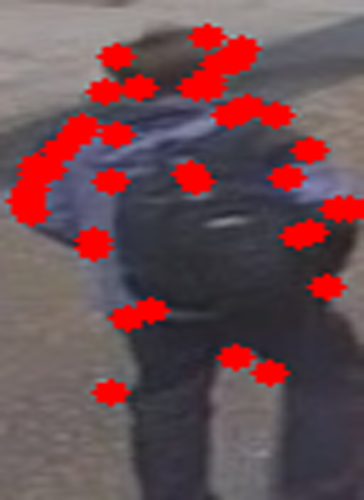
\includegraphics[width=5cm]{changeCamera/tomeuTetx.png}}
\subfigure[Low texture person.]{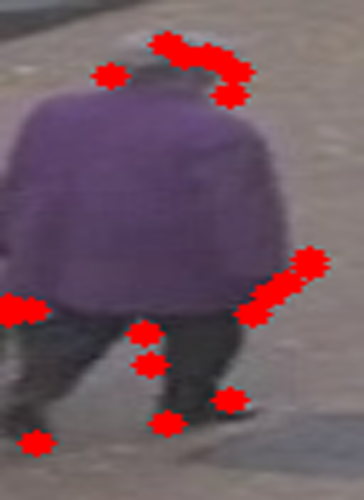
\includegraphics[width=5cm]{changeCamera/donaTetx.png}}
\subfigure[Far away person.]{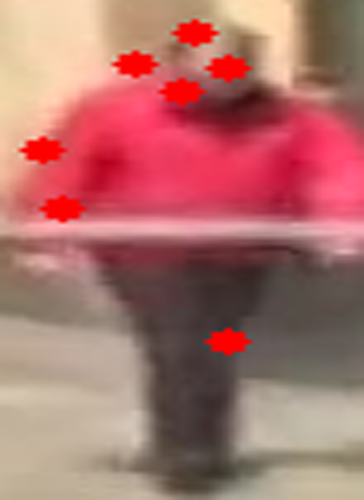
\includegraphics[width=5cm]{changeCamera/foto004.png}}
\caption{Differences texture examples.}
\label{Fails1}
\end{figure}








\section{Future work}


This is a first entrance on trackings algorithm, we have a resanoable results. We can add some details to improve our results.


\begin{itemize}

\item Port to C++. We used a srcipting programming languagge, if we switch to a compiled programing language we would increase the time perfomance.

\item GPU implementation. Computing displacement for each tracket could be computed in a parallel way. They are independent from each other and are a low demanding. 

\item Propbabilistic framework. Include bayesian filter techniques to increase perfomance.

\item Siamese architectures. Study new siamese architecture to increase the accuracy of this modeule, like inception stem of InceptionV3 or include the optical flow information in the neural network.

\item Data association. Use much confidence techniques to associate the detections, the current methods relay ond probablistic graphical models.

\end{itemize}
